\chapter{Metodi e Modelli per lo sviluppo di applicazioni Mobile}
La scelta di seguire un determinato schema progettuale di una applicazione è stata fatta in base alle conoscenze apprese durante la mia esperienza di tirocinio in azienda, durante la quale non mi sono occupato dell'intera progettazione dell'applicazione, mi occupavo solo dello sviluppo \emph{frontend} di questa, ma per uno sviluppatore è necessario conoscere l'intera dinamica che si svolge all'interno di essa anche se non andrà a intervenire su determinate parti.\\

La politica che è stata intrapresa in azienda è stata quella della \emph{Separation of Concernes}(SoC), che in italiano si traduce in \emph{Separazione dei Compiti}. Si tratta di un principio di design dell'applicazione per dividere l'applicazione in sezioni distinte, e ad ogni sezione assegnare un particolare compito o risoluzione di un problema. Questa scelta progettuale introduce il concetto di \emph{modulo} di una applicazione, ovvero l'applicazione poi dipenderà dai moduli che andremo a creare e ad unire tra di loro. I moduli ragionevolmente saranno indipendenti uno dall'altro in modo tale da garantirne l'integrità e il loro re-utilizzo.\cite{wiki:soc}\\
Il concetto appena visto astrae molto da una applicazione vera e propria, sta a chi la progetta decidere con che granularità  e se è veramente necessario applicarlo. Dato che parliamo di tecnologie web, un chiaro esempio si separazione dei compiti è quello della struttura di una pagina web, divisa in HTML per la struttura, CSS per lo stile, e Javascript per la logica e comportamento.\\

In questo capitolo andremo a vedere in che modo i compiti si possono separare all'interno di una applicazione, e quali strutture e/o design pattern possono risultare utili per lo sviluppo.
 
\section{Design Patterns}

Quando si progetta una applicazione risulta molto utile utilizzare schemi architetturali e metodologici che rendono da un lato l'applicazione efficiente dall'altro una scrittura del codice molto chiara e modulare facile da correggere nel caso di eventuali errori. I design pattern vengono in aiuto a questa esigenza del programmatore.

\emph{In informatica, nell'ambito dell'ingegneria del software, un design pattern (traducibile in lingua italiana come schema progettuale, schema di progettazione, schema architetturale), è un concetto che può essere definito "una soluzione progettuale generale ad un problema ricorrente". Si tratta di una descrizione o modello logico da applicare per la risoluzione di un problema che può presentarsi in diverse situazioni durante le fasi di progettazione e sviluppo del software, ancor prima della definizione dell'algoritmo risolutivo della parte computazionale.}
\hspace*{\fill}\cite{wiki:design_pattern} 

Il problema ricorrente che si ha nello sviluppo di applicazioni e quello della decisione di dove debbano stare determinati compiti / operazioni / sezioni all'interno dell'applicazione. Ad esempio la separazione della parte dell'interfaccia da quella dedicata alla manipolazione dei dati da quella dedicata alla memorizzazione. Dividere i vari compiti di una applicazione può risultare molto produttivo, in quanto si possono sviluppare in parallelo diverse parti dell'applicazione senza influire sulle altre e volendo con la possibilità di utilizzare tecnologie differenti.

Durante il periodo di tirocinio presso l'azienda \emph{BigThink SRL} per la creazione di Web Applications sono stati utilizzati pattern come : Client-Server, SoC, Frontend e Backend gli altri design pattern che verranno introdotti sono necessari per comprendere meglio alcune tecnologie che verranno utilizzate.
 
\subsection{Frontend e Backend}
Queste due parole sono spesso usate in informatica in molti ambiti, nel contesto specifico dell'applicazione \texttt{frontend}(in italiano parte davanti) denota quella parte dell'applicazione responsabile di gestire l'interfaccia utente e i dati provenienti da essa, mentre \texttt{backend}(in italiano parte dietro) indica la sezione dell'applicazione dedita alla gestione dei dati provenienti dalla parte frontend. L'interazione che hanno le due parti è un chiaro esempio di interfaccia.\\
\textbf{Frontend:} questa è la parte caratteristica dell'applicazione, in quanto ne definisce il comportamento e l'aspetto, determinando la logica con cui si evolverà al rapporto con l'utente. A differenza della parte \emph{backend} questa non definisce nessuna manipolazione dei dati ma solo la loro rappresentazione(vista) determinando transizioni e/o animazioni.
Nella parte \emph{frontend} è inclusa anche la fase di definizione estetica dell'interfaccia, ma spesso questa spetta a una figura professionale distinta atta "vestire" l'applicazione.
\textbf{Backend:} questa parte è completamente diversa dalla prima, in quanto definisce la manipolazione dei dati all'interno dell'applicazione ma non da nessuna informazione caratteristica di essa. In particolare fornisce dei servizi ai quali la parte \emph{frontend} può accedere e recuperare/fornire dei dati, come ad esempio l'autenticazione di un utente a un servizio. Tutta la gestione dei dati che viene fatta da questa parte, viene oscurata alla parte \emph{frontend} per garantire un servizio di sicurezza molto elementare, in modo tale che se l'utente inserisce dei dati errati che vengono passati dalla parte \emph{frontend} a quella \emph{backend}, in modo errato, nessuna operazione verrà eseguita e l'integrità dei dati preservata.\\

A livello professionale molti sviluppatori si identificano appunto come \emph{frontend} e/o \emph{backend} developer per appunto identificarsi specializzati nello sviluppo di una parte specifica dell'applicazione.
Il vantaggio di usare un approccio di questo tipo sta nel fatto che la parte \emph{frontend} è l'unica specifica per una data applicazione. Se la parte \emph{backend} viene progettata bene, e possibile utilizzare i servizi che fornisce anche in futuro da altre applicazioni, pur seguendo il protocollo che richiede. Inoltre a livello professionale si può procedere parallelamente nello sviluppo delle parti in modo tale da ottimizzare i tempi, pur seguendo uno schema stabilito a priori.\\

\subsection{Pattern Client-Server}
\textbf{Definizione:} Il modello client-server è un modo per strutturare applicazioni distribuite che distingue due parti di un processo di comunicazione, la prima che fornisce una risorsa e/o un servizio chiamata server, la seconda che analogamente li può richiedere, chiamata client. La comunicazione in generale avviene attraverso la rete, ed è il client a iniziarla. Il compito del server è quello di predisporre le risorse che ha ai vari client che li chiedono, rimanendo appunto "in ascolto", il client invece non condivide le risorse con altri, può solo interagire con il server\cite{wiki:cliserv}.\\

Come si può già intuire le parti che verranno prese in questo modello saranno rispettivamente quella del \emph{frontend} e quella del \emph{backend}. Specificatamente nell'ambito delle applicazioni i client saranno le varie istanze della parte \emph{frontend} dell'applicazione sui vari dispositivi, mentre il server, fornitore di servizi, conterrà la parte di \emph{backend}.

\subsection{Mustache}

In ambito web può essere utile un sistema di template che aiuti a separare la logica dalla presentazione dei dati(metodologia molto in voga tra le tecnologie web).

\emph{Mustache è un web template system con una implementazione disponibile in molti linguaggi(sarà utili quella in Javascript). Mustache è descritto come un sistema senza logica, in quanto manca qualsiasi dichiarazione di controllo del flusso esplicita, ovvero istruzioni condizionali e di iterazione. Il tutto può essere implementato tramite un sistema di tag, liste procedurali e lambda}
\hspace*{\fill}\cite{wiki:mustache}

\subsection{MVC Pattern}
\label{sec:MVC}
\emph{Il Model-View-Controller pattern (MVC) in informatica, è un pattern architetturale molto diffuso nello sviluppo di sistemi software, in particolare nell'ambito della programmazione orientata agli oggetti, in grado di separare la logica di presentazione dei dati dalla logica di business.}

Il pattern è basato sulla separazione dei compiti fra i componenti software che interpretano tre ruoli principali:
\begin{description}
\item[model] fornisce i metodi per accedere ai dati utili all'applicazione;
\item[view] visualizza i dati contenuti nel model e si occupa dell'interazione con utenti e agenti;
\item[controller] riceve i comandi dell'utente (in genere attraverso il view) e li attua modificando lo stato degli altri due componenti.
\end{description}
Questo schema, fra l'altro, implica anche la tradizionale separazione fra la logica applicativa (in questo contesto spesso chiamata "logica di business"), a carico del controller e del model, e l'interfaccia utente a carico del view.
\hspace*{\fill}\cite{wiki:mvc}

\subsection{MVVC Pattern}
\emph{Il Model-View-ViewModel è un pattern architetturale basato sul pattern MVC e MVP che tenta di separare più chiaramente lo sviluppo di interfacce utente (UI) da quello della logica di business e il comportamento in un'applicazione . A tal fine, molte implementazioni di questo modello fanno uso di associazioni dati dichiarativa(data bindings) per consentire una separazione di lavoro su Vista da altri livelli.}

Questo facilita l'interfaccia utente e lo sviluppo che si verificano quasi contemporaneamente all'interno dello stesso codice. Gli sviluppatori dell'interfaccia utente scrivono associazioni verso il ViewModel nel documento di markup (HTML) mentre il Model e il ViewModel sono mantenuti da altri sviluppatori che lavorano sulla logica dell'applicazione(business logic).

\hspace*{\fill}\cite{book:mvvm}
\section{API}

\emph{In informatica le API(Application Programming Interface) sono un insieme di operazioni, protocolli, strumenti per lo sviluppo del software. Una API rappresenta una specifica componente del software in termini di operazione, input, output e tipi soggiacenti. Una API definisce funzionalità totalmente indipendenti dalla loro rispettiva implementazione, il che consente di poter variare rispettivamente l'implementazione e la definizione senza che una influisca sull'altra. Una buona API rende più facile lo sviluppo del software fornendo vari "mattoni" con cui poter sviluppare il software, il ruolo del programmatore è quello di unire i vari blocchi richiesti.}
\hspace*{\fill}\cite{wiki:api}

Un primo esempio di API è già stato menzionato quando si è parlato dei framework per lo sviluppo ibrido. In quel caso le API erano fornite tramite Javascript in modo tale che potessero essere interpretate all'interno di un contenitore nativo che potesse interpretare linguaggi web(come un browser). In questo caso i blocchi di cui si parla sono le rispettive API che consentono di comunicare con le funzionalità del dispositivo come ad esempio la fotocamera, il gps, la vibrazione, l'accelerometro ecc\ldots.

L'utilizzo di API è stato fatto durante il mio tirocinio aziendale per lo scambio di dati tra la parte Frontend e Backend di Web Application, in particolare sono state utilizzate delle API REST.

\subsection{API Rest}

\textbf{Re}presentational \textbf{S}tate \textbf{T}ransfer (REST) è uno stile di architettura software per sistemi distribuiti. Un sistema conforme ai principi di design REST è detto RESTful. Il Web è l'esempio più importante e più famoso di sistema distribuito che realizza i principi REST. D'altra parte non è un caso. Infatti Roy Fielding, il padre di REST, introdusse per la prima volta l'espressione Representational State Transfer nella sua tesi di dottorato per indicare le caratteristiche delle parti meglio progettate del Web.
Il termine REST è diventato più comune negli ultimi anni con l'esplosione del Web 2.0 e il proliferare di servizi web.
In poche parole un'architettura RESTful è di tipo client / server. I client fanno richieste ai server che a loro volta processano le richieste e restituiscono una risposta. Richieste e risposte contengono delle rappresentazioni di risorse. Una \textbf{risorsa} è un concetto significativo per il dominio di riferimento (ad esempio l'articolo di un blog o il profilo utente di un social network) che può essere identificato attraverso un indirizzo. Una \textbf{rappresentazione} è una descrizione dello stato corrente o voluto di una risorsa.

\begin{figure}[htbp]
  \centering
    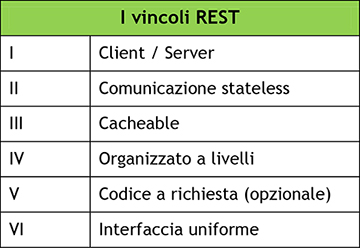
\includegraphics[scale=0.75]{Figures/tab-rest.jpg} 
    \rule{35em}{0.5pt}
  \caption[Vincoli REST]{Vincoli che una applicazione deve rispettare per essere considerata RESTful}
  \label{fig:REST Rules}
\end{figure}

Lo stile architetturale REST descrive 6 vincoli (cinque più uno facoltativo) che devono essere rispettati da un sistema affinché possa essere definito RESTful (tabella \ref{fig:REST Rules}). Poiche’ REST è uno stile e non una tecnologia e nemmeno una lista di raccomandazioni tecniche, i dettagli su come questi vincoli debbano essere implementati sono lasciati ai singoli sviluppatori. Ad esempio, l'Application Layer sul quale costruire il sistema non deve essere per forza HTTP, anche se HTTP è quasi sempre la scelta più naturale. Il formato delle rappresentazioni delle risorse spesso è XML o JSON, ma potrebbe essere anche PDF. Infine REST non è uno stile architetturale solo per le web application, ma è molto più generale. Se i vincoli REST sono rispettati, l’architettura software di un robot (server) controllato da uno o più computer (client) dove le risorse sono l’hardware del robot (sensori e motori) può essere a tutti gli effetti considerata RESTful.
L'esperienza ha mostrato che sistemi RESTful hanno delle desiderabili proprietà emergenti, come ad esempio la scalabilità e la modificabilità.
Un esempio di organizzazione delle risorse nel protocollo REST:

\begin{lstlisting}[language=php, caption = {Esempio di API REST generica}, label = {lst:genericRESTAPI}]
	/{tipo di risorsa}/{id della risorsa}/{azione}
\end{lstlisting}

applicando l'esempio nel contesto dei blog:

\begin{lstlisting}[language=php, caption = {Esempio di API REST nel caso di un ipotetico blog} , 
				   lablel = {lst:blogRESTAPI}]
	/posts/1/edit oppure /posts/1/view
\end{lstlisting}

\subsection{Chiamate XHR}

